\chapter{Results}
	\section{Imaging Excited-State Dynamics}
		The following article focusses on imaging and characterising the dynamics using femtosecond spectroscopy and time-dependent density functional theory. Specifically on the idea of a fall-back time, which is defined as the time delay $\tau\vcentcolon=t_{ion}-t_{exc}$ between the time instance of the photo-excitation of Rb to the 5p and 6p states, and the time instance of its photo-ionisation, such that the Rb cation is still solvated by the helium droplet.
		
		The experimental setup used is very similar to the one introduced in the the previous section. To probe the alkali, time-resolved imaging spectroscopy in a so called ``pump-probe'' scheme has been used. In this setup---after the droplet has picked up the alkali---a first laser, the pump, is used to bring the alkali in an excited state. This laser can be tuned to various different excitation wavelengths $\lambda_{exc}$. A variable time delay $\tau$ later a second laser, the probe, is used to ionise the alkali. The time delay can be chosen on a femtosecond time scale. The subsequent photo-electrons and photo-ions are then led into a velocity map imaging detector\citep{Eppink1997} to visualise their velocity distributions which in turn gives us detailed information about the energies involved in the studied process.
		
		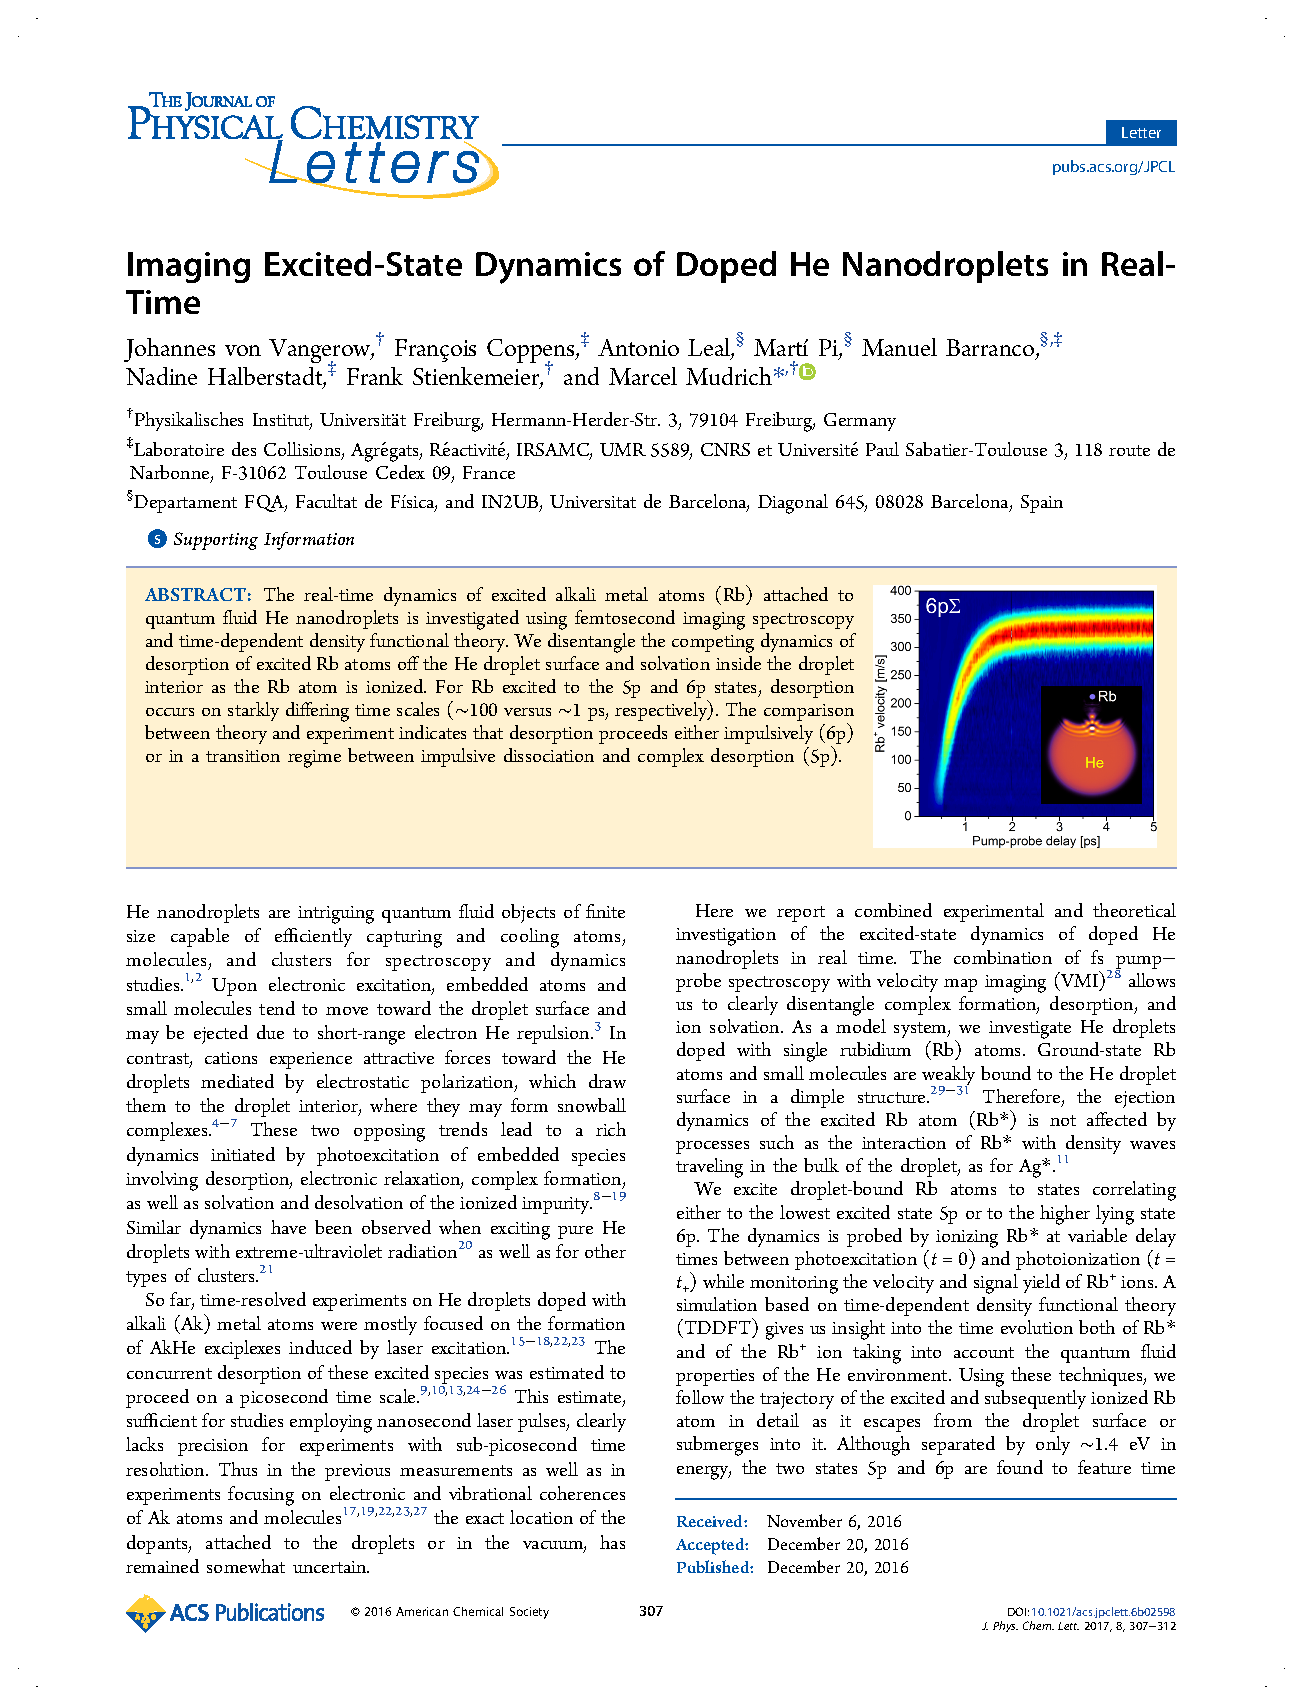
\includepdf[pages=-, scale=0.875, pagecommand={}]{jpcl_vol8_no1_pp307-312.pdf}
		\cleardoublepage

	\section{Desorption dynamics of RbHe exciplexes}
		How do we resolve the discrepancy between the experimental observation that Rb atoms---excited to the 5p$\,^2\Pi_{3/2}$ state---detach from the droplet's surface, and TD-DFT simulations that show that they result in a surface-bound state? That is the question that led to this work. Upon photo-excitation of Rb to the 5p$\,^2\Pi_{3/2}$ state, a He atom may be attached to it forming a HeRb exciplex; this cannot happen if Rb is excited to the 5p$\,^2\Pi_{1/2}$ state because it finds a barrier (see Figure \ref{fig:potentials}) preventing exciplex formation.

		\begin{figure}[t]
			\begin{center}
				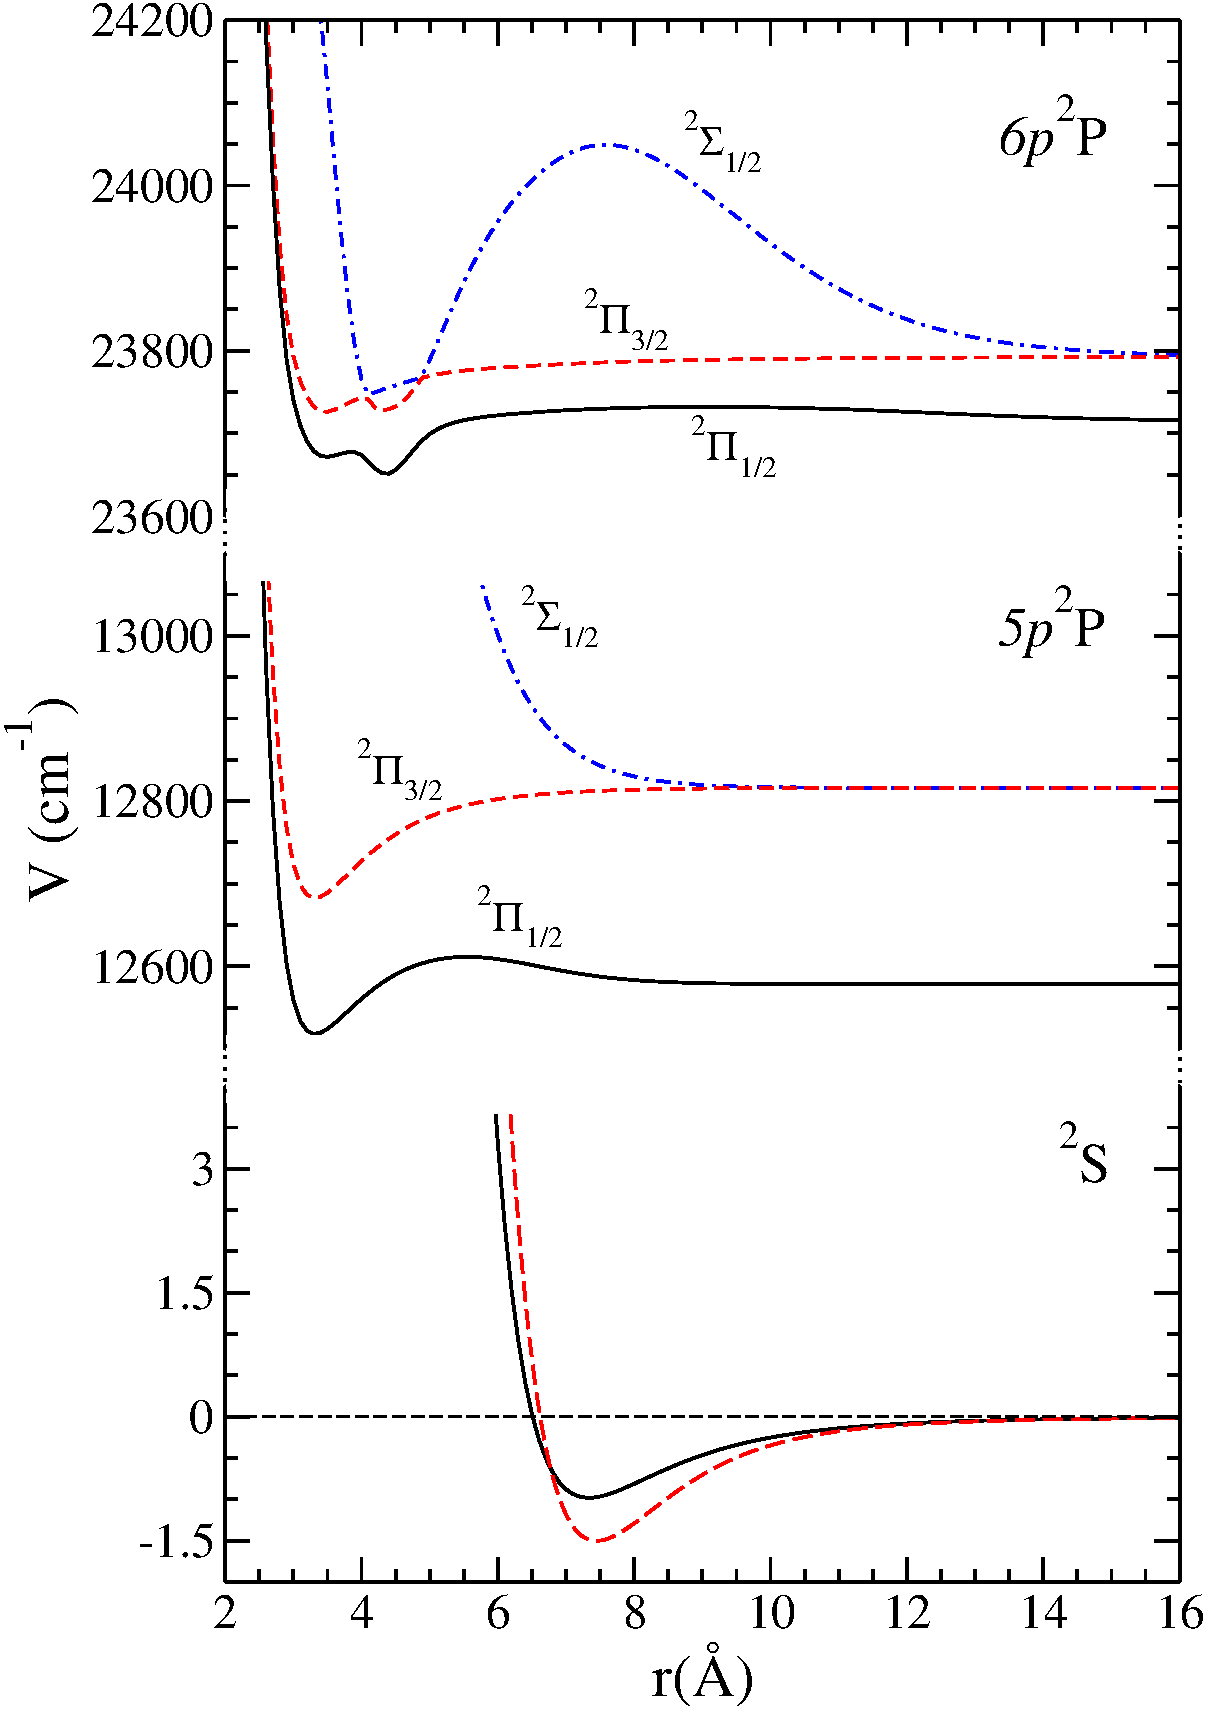
\includegraphics[width=\textwidth]{potentials}
			\end{center}
			\caption{$^2$S, 5p$\,^2$P, and 6p$\,^2$P Rb-He pair potentials used in this work. The splitting introduced by the spin-orbit interaction has been included. The $^2$S He-Rb pair potential of Ref. \citen{Pas83} is also displayed (bottom dashed line).}
			\label{fig:potentials}
		\end{figure}
		
		In the gas phase, a HeRb 5p$\,^2\Pi_{1/2}$ exciplex can be formed if there is enough kinetic energy for Rb* to overcome the potential barrier; alternatively, the collision of the HeRb 5p$\,^2\Pi_{3/2}$ exciplex with another atom or complex might relax the Rb* atom from the 5p$\,^2\Pi_{3/2}$ to the 5p$\,^2\Pi_{1/2}$ state, overcoming the barrier as the potential wells for both states are at similar Rb-He distances. In the condensed (droplet) phase at 0.4 K temperature, neither of these mechanisms are available to explain the formation of HeRb 5p$\,^2\Pi_{1/2}$ exciplexes and their potential ejection.

		However, another possible way for this to happen is non-radiative de-excitation from the 5p$\,^2\Pi_{3/2}$ to the 5p$\,^2\Pi_{1/2}$ that populates the latter state and leaves the Rb* atom with enough kinetic energy so as to be ejected. Notice from Figure \ref{fig:potentials} that the minimum of the 5p$\,^2\Pi_{3/2}$ potential is 12683 cm$^{-1}$, and that of the 5p$\,^2\Pi_{1/2}$ potential is at 12518 cm$^{-1}$; the value of this potential at the barrier is 12611 cm$^{-1}$. Thus, non-radiative de-excitation of the Rb* atom may add to its original kinetic energy of up to 165 cm$^{-1}$. It is worth noting that it will be ejected in the 5p$\,^2\Pi_{1/2}$ state, and not in the 5p$\,^2\Pi_{3/2}$ it was previously photo-excited to.
		
		This publication contains a extension of our combined experimental and theoretical investigation presented in the previous section. Here we focus on the formation of free RbHe-exciplex molecules from laser-excited Rb-doped He nanodroplets through the mechanism of electronic spin relaxation.% The role of relaxation of internal degrees of freedom of the RbHe exciplex in the desorption process has not been explicitly addressed.	

		\cleardoublepage
		\includepdf[pages={-}, scale=0.8, pagecommand={}]{pccp_vol20_no14_pp9309-9320.pdf}
		
	\section{Supervised work: potassium-doped nanodroplets}
		Under the supervision of Nadine Halberstadt and me, a master research internship --- \emph{M2 Physique Fondamentale} --- titled ``\emph{\textbf{Dynamics of a superfluid helium nanodroplet doped with a single potassium atom}}'' has been performed by Maxime Martinez.
	
		The project investigates the static and dynamic behaviour of a single potassium (K) atom excited from the K-$^4$He$_{1000}$ equilibrium configuration to the K*(4p)-$^4$He$_{1000}$ and K*(5s)-$^4$He$_{1000}$ states. The choice of potassium was motivated by a discrepancy in the time-resolved experimental studies\citep{Schulz2001,Reho2000-1,Reho2000-2}. Moreover, the mass of potassium sits between those of the heavier alkalis like rubidium and cesium, and the lighter ones, like lithium and sodium. Therefore, potassium presents an interesting case, being on the borderline between the classical regime for heavy alkalies and a quantum--mechanical regime for the lighter ones. Both treatments of the equilibrium properties and the 5s$\leftarrow$4s excitation are studied. This work is not included in the thesis but can be found in \rf{Martinez2017}.
		
		It is concluded that quantum effects of K do exist but are not essential to the understanding and description of the dynamics. Therefore the K*(4p)-$^4$He$_{1000}$ excitation is studied with a classical description of K.
